\subsection{A Transaction Optimization Framework}\label{sec:tx_optimization_framework}

We now identify different phases in the transaction optimization process; in
a hypothetical \emph{transaction optimizer} each phase would be a distinct
module. These phases are different approaches to producing equivalent
transactions. The phases operate on three levels of optimization:
\begin{inparaenum}[a)]
    \item a declarative (rule-based) level,
    \item a logical/algebraic (cost-based) level, and
    \item a physical/algorithmic (cost-based) level,
\end{inparaenum}
as depicted in Figure~\ref{fig:optimization-phases}. The input of the process
is a transaction set $[\tx_x]$, that we want to optimize, and while output is the
optimal transaction $\tx_{x-Optimal}$.

\paragraph{Rules}
This phase is declarative, as it does not depend on the cost; instead, when
applied, it necessarily produces a better transaction. Essentially it consists
of \emph{heuristic rules} that are applied by default to produce an equivalent
transaction; example of such rules are ``create a single output per address''
or ``consume as many inputs and create as few outputs as possible''.

\paragraph{Algebraic Transformations}
These are transformations at the level of logical operators that define a
transaction's execution. Generally the efficiency of such transformation is
evaluated based on the entailed cost. Examples of such transformations are the
2-for-1 transformation (cf. Definition~\ref{def:2-for-1}) and different
transaction orderings (cf. Definition~\ref{def:subtransaction}).

\paragraph{Methods and Structures}
This phase optimizes the algorithm that implements a logical operator. For
instance, given two algorithms $A, B$ result in transaction costs $\cost_A, \cost_B$,
if $\cost_A < \cost_B$ we would choose $A$; one such example is the different
implementations of the input selection operator $\sigma$, as shown in
Figure~\ref{fig:3-logical-plans}. Optimizations in this phase may also change
the data structure used to access the underlying data, which in our case is the
ledger state.

\paragraph{Planning and Searching}
This phase employs a \emph{searching strategy} to explore the available space
of candidate solutions, \ie equivalent transaction plans. This space consists
of the transactions produced from the above phases, each evaluated based on
their cost, under the available cost model.

\begin{figure}[h!]
	\centering
	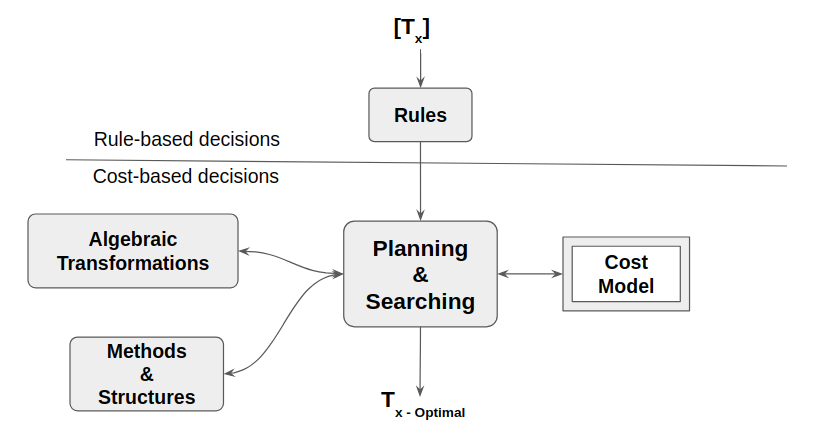
\includegraphics[width=0.8\columnwidth,keepaspectratio]{figures/utxo_growth/optimization_phases.png}
	\caption{The transaction optimization process.}
	\label{fig:optimization-phases}
\end{figure}

\subsection{Transaction Optimization Techniques}\label{sec:tx_optimization_techniques}

In this section, we propose three transaction optimization techniques
based on the aforementioned optimization levels:
\begin{inparaenum}[a)]
    \item heuristic rule-based,
    \item logical/algebraic transformation cost-based, and
    \item physical/algorithmic cost-based.
\end{inparaenum}

\subsubsection{Input Selection Optimization}\label{sec:input_sel_optimization}

We demonstrate this technique with an example. Assume Alice wants to give Bob
$5$ coins. Figure~\ref{fig:3-logical-plans} depicts three equivalent
transactions for implementing this payment. Observe that each plan is
represented as a tree, where the intermediate nodes are the previously defined
logical operators (that act on a ledger state) and the leaf nodes are ledger
states. We also assume that the state cost is the number of elements (UTxOs) in
the state.  The three transactions have the same structure, \ie they are the
same logical expression, but result to different ledger states with different
costs. The transactions differ only in the output of the input selection
operator ($\sigma_{(Alice, 5)}$), a difference which may be attributed to
different implementations of the operator.

\begin{figure}[h!]
    \centering
    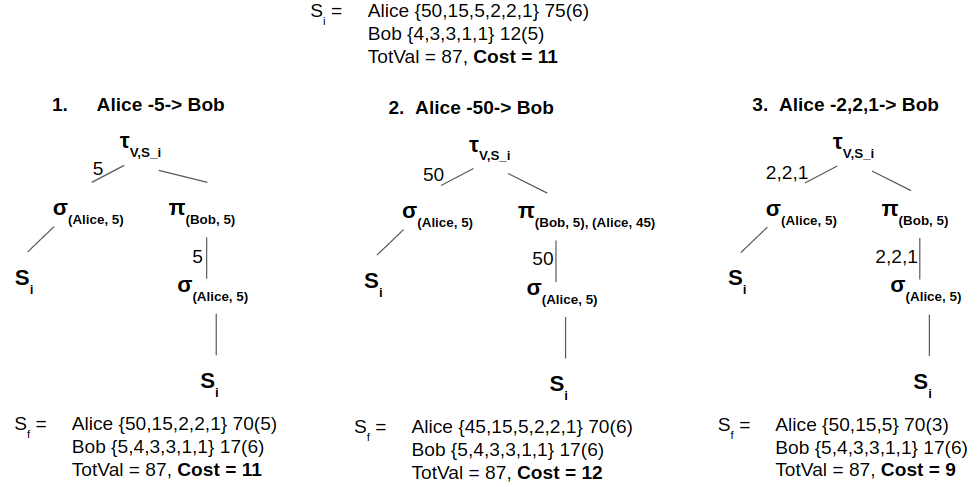
\includegraphics[width=1\columnwidth,keepaspectratio]{figures/utxo_growth/3-logical-plans.png}
    \caption{An example of three equivalent transactions that transfer 5
    tokens from Alice to Bob but incur different state costs.}
    \label{fig:3-logical-plans}
\end{figure}

\subsubsection{The 2-for-1 Transformation}\label{sec:2-for-1}

We again consider the example where Alice wants to give Bob $5$ coins.
Figure~\ref{fig:4th_logical_plan.png} depicts a fourth, more complex,
equivalent transaction. This transaction consists of two subtransactions (cf.
Definition~\ref{def:subtransaction}), where Alice first gives Bob $17$ coins
and then receives $12$.
When the first transaction is completed, an intermediate state ($S'_i$) is
created, which is then given as input to the second transaction, that produces
the final ledger state $\ledgerState_f$ of cost $3$. Observe that, although
more complex, this transaction minimizes the final ledger state ($72\%$ cost
reduction). Intuitively, this transaction spends all of Alice's outputs with
the first sub-transaction and then does the same for Bob with the second
sub-transaction. Therefore, the optimal cost does not depend on input selection
(like
the 3rd plan of Figure~\ref{fig:3-logical-plans}), but requires the combination
of two transactions that implement a single payment, under a specific
amount ($12$). Definition~\ref{def:2-for-1} provides a formal specification of
the \emph{2-for-1} logical (algebraic) transformation.

\begin{figure}[h!]
    \centering
    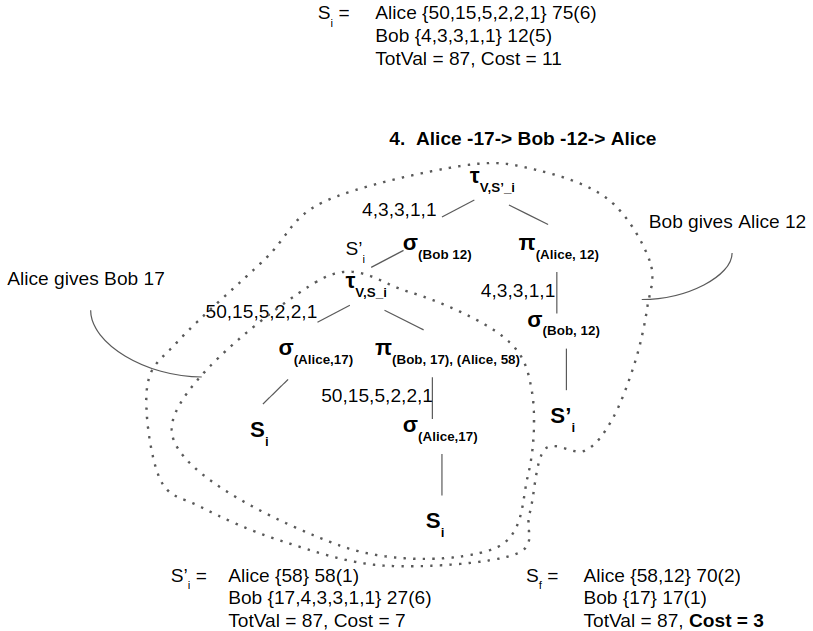
\includegraphics[width=0.9\columnwidth,keepaspectratio]{figures/utxo_growth/4th_logical_plan.png}
    \caption{A 2-for-1 transaction that transfers 5 tokens from Alice to Bob.}
    \label{fig:4th_logical_plan.png}
\end{figure}

\begin{definition}\label{def:2-for-1}
        Given a transaction $\tau_1$, which transfers an amount $V$ from party
        A to B, the algebraic \emph{2-for-1} transformation creates an
        equivalent transaction $\tau_2$, which consists of
        \begin{inparaenum}[(a)]
            \item a subtransaction, which transfers $V+V_c$ from party A to B and
            \item an outer transaction, which transfers $V_c$ from party B to A.
        \end{inparaenum}
\end{definition}

Figure~\ref{fig:2-for-1} depicts the 2-for-1 algebraic transformation based on
an amount $V_c$. To
implement such a scheme we require an \emph{atomic operation}, where the
grouped transactions are executed simultaneously. One method to implement the
atomic transfers is CoinJoin~\cite{coinjoin}, which was proposed for increasing
the privacy in Bitcoin; in CoinJoin, the transaction is constructed and signed
gradually by each party that contributes its inputs. A similar concept is
Algorand's atomic transfers \cite{atomictransfers}, that achieves atomicity by
grouping transactions under a common id.

\begin{figure}[h!]
	\centering
	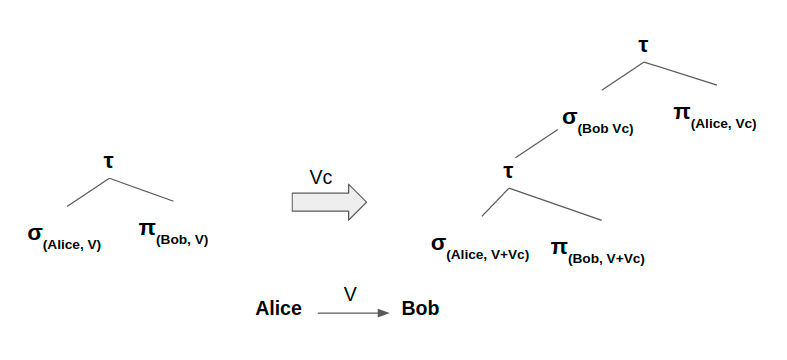
\includegraphics[width=0.9\columnwidth,keepaspectratio]{figures/utxo_growth/2-for-1.png}
	\caption{The 2-for-1 algebraic transformation.}
	\label{fig:2-for-1}
\end{figure}

Intuitively, 2-for-1 reduces the transaction's cost by also consuming UTxOs of
the receiving party, instead of only consuming outputs of the sending party.
Specifically, assume the initial state $\ledgerState_i = \{|A|, |B|\}$, where
$|A|$ denotes the number of outputs owned by party A. When issuing a payment to
B, party A can consume all outputs and consolidate its remaining value to a
single UTxO, the ``change'' output. Such transaction results in state
$\ledgerState_f = \{1, |B|+1 \}$ with cost $cost(\ledgerState_f) = |B|+2$.
If we apply the 2-for-1 transformation, the final state is $\ledgerState_f' =
\{1+1, 1\}$ with a cost of $cost(\ledgerState_f') = 3$; if $|B| > 1$, then
$cost(\ledgerState_f') < cost (\ledgerState_f)$.  Therefore, if the receiving
party has multiple outputs, this transformation creates a transaction with a
smaller cost. Consequently, by giving the opportunity to the receiving party of
a transaction to spend also its outputs, the 2-for-1 transformation
\emph{always} results in a greater shared state cost reduction than the
individual un-transformed transaction in the case where there are no fee
constraints and thus outputs can be spent freely; otherwise it is a cost-based
decision.

\subsubsection{Transaction Total Ordering and the Last-Payer Heuristic Rule}

Assume the following four transactions:
\begin{inparaenum}[(1)]
    \item $T_1$: Alice $\xrightarrow{V_1}$ Charlie,
    \item $T_2$: Bob $\xrightarrow{V_2}$ Charlie,
    \item $T_3$: Eve $\xrightarrow{V_3}$ Alice, and
    \item $T_4$: Eve $\xrightarrow{V_4}$ Bob,
\end{inparaenum}
which are applied on an initial ledger state $\ledgerState_i = \{|Alice| = 5,
|Bob| = 5, |Charlie| = 2, |Eve| = 3\}$ with cost $cost (\ledgerState_i) = 15$;
as before, $|A|$ denotes the number of outputs owned by party A and the state
cost is the number of all UTxOs.

A first execution order is as follows: $T_1 \rightarrow T_2 \rightarrow T_3
\rightarrow T_4$. For simplicity and without loss of the generality, we assume
that when a party pays, it always consumes all available outputs, thus having
with a single output afterwards (the leftover balance). Similarly, when a party
gets paid, the number of UTxOs that it owns increases by one. Next, we describe
the ledger state changes each transaction is executed:
\begin{math}
    \\
    \ledgerState_i = \{|Alice| = 5, |Bob| = 5, |Charlie| = 2, |Eve| = 3\}, cost = 15\\
    T_1: \{|Alice| = 1, |Bob| = 5, |Charlie| = 3, |Eve| = 3\}, cost = 12\\
    T_2: \{|Alice| = 1, |Bob| = 1, |Charlie| = 4, |Eve| = 3\}, cost = 8\\
    T_3: \{|Alice| = 2, |Bob| = 1, |Charlie| = 4, |Eve| = 1\}, cost = 8\\
    T_4: \{|Alice| = 2, |Bob| = 2, |Charlie| = 4, |Eve| = 1\}, cost = 9\\
\end{math}

Assuming a different order, $T_3 \rightarrow T_4 \rightarrow T_1
\rightarrow T_2$, the state changes as follows:

\begin{math}
	\\
	\ledgerState_i = \{|Alice| = 5, |Bob| = 5, |Charlie| = 2, |Eve| = 3\}, cost
	= 15\\
	T_3: \{|Alice| = 6, |Bob| = 5, |Charlie| = 2, |Eve| = 1\}, cost = 14\\
	T_4: \{|Alice| = 6, |Bob| = 6, |Charlie| = 2, |Eve| = 1\}, cost = 15\\
	T_1: \{|Alice| = 1, |Bob| = 6, |Charlie| = 3, |Eve| = 1\}, cost = 11\\
	T_2: \{|Alice| = 1, |Bob| = 1, |Charlie| = 4, |Eve| = 1\}, cost = 7\\
\end{math}

Evidently, the different execution order results in different resulting state
cost. Therefore, by changing the nesting order of the transactions in an
expression tree, different plans may conduct the same payment with different
cost.

Intuitively, parties should have the ability to consume outputs that are
produced by the other transactions. For instance, regarding $T_1$ and $T_3$,
the order $T_3 \rightarrow T_1$ is more cost effective ($cost = 10$) than $T_1
\rightarrow T_3$ ($cost = 11$), since Alice can consume the output created by
Eve. Specifically, if in the last transaction where $\party$ participates,
either as a sender or a receiver, $\party$ is the sender, then it can minimize
its state cost; we call this the \emph{last-payer heuristic rule}.
